% FDD in IEEE 9-Bus System Beamer Presentation
\documentclass{beamer}
\usepackage[english]{babel}
\usetheme{KFUPM}

\usepackage{svg}
\usepackage[utf8]{inputenc}
\usepackage[T1]{fontenc}
\usepackage{transparent}
\usepackage{amsmath}
\usepackage[document]{ragged2e}
\usepackage{svg}
\usepackage{algorithmic}
\usepackage{algorithm}
\usepackage{multirow}
%% Use any fonts you like.
\usepackage{helvet}
\usepackage{booktabs}

% GRAPHICS AND FLOATS
% ------------------------------------------------------------------------------
\usepackage{graphicx}
\usepackage{subcaption}
\usepackage{float}
\usepackage{tikz}
\usetikzlibrary{shapes, arrows.meta, positioning}
\usetikzlibrary{shapes.geometric, arrows, positioning}
\usepackage{pgf-pie}
\usepackage{makecell}



% Math
\usepackage{amsmath, amssymb}

% Font formatting (optional, for small caps, etc.)
\usepackage{lmodern}

% Text color (if using custom colors)
\usepackage{xcolor}
% ------------------------------------------------------------------------------


\title{\textcolor{white}{\bf Title}}
\subtitle{\textcolor{white}{\tiny \transparent{0.7} Project N. }}
\author{{\it \tiny \transparent{0.7} By:}\\ Name}
\date{{\tiny \today}}
\institute{{\it \tiny \transparent{0.7} Supervisor:}\\ \tiny Dr. Name}


\begin{document}

    % Title Slide
    \begin{frame}[plain,t]
        \titlepage
    \end{frame}

    \begin{frame}
  \frametitle{\textcolor{white}{\bf Outline}}
  \textcolor{white}{
    \tableofcontents
  }
\end{frame}

    \section{Introduction}

\begin{frame}
  \frametitle{\textcolor{white}{\bf Introduction}}
  \textcolor{white}{
    \begin{itemize}
        \item write here.
    \end{itemize}
  }
\end{frame}

    % \subsection{Problem Statement \& Motivation}

\begin{frame}
  \frametitle{\textcolor{white}{\bf Problem Statement \& Motivation}}
  \textcolor{white}{
    \begin{itemize}
        \item write here
    \end{itemize}
  }
\end{frame}

    % \subsection{Objectives \& Scope}

\begin{frame}
  \frametitle{\textcolor{white}{\bf Objectives \& Scope}}
    \textbf{Objectives:}
    \begin{itemize}
        \item ...
    \end{itemize}
    
\end{frame}

\begin{frame}
  \frametitle{\textcolor{white}{\bf Objectives \& Scope}}

    \textbf{Scope of the Study:}
    \begin{itemize}
        \item .....
    \end{itemize}
\end{frame}


    \section{Methodology}

\begin{frame}{Methodology}

    \begin{figure}[h!]
        \centering
        \scalebox{0.8}{
        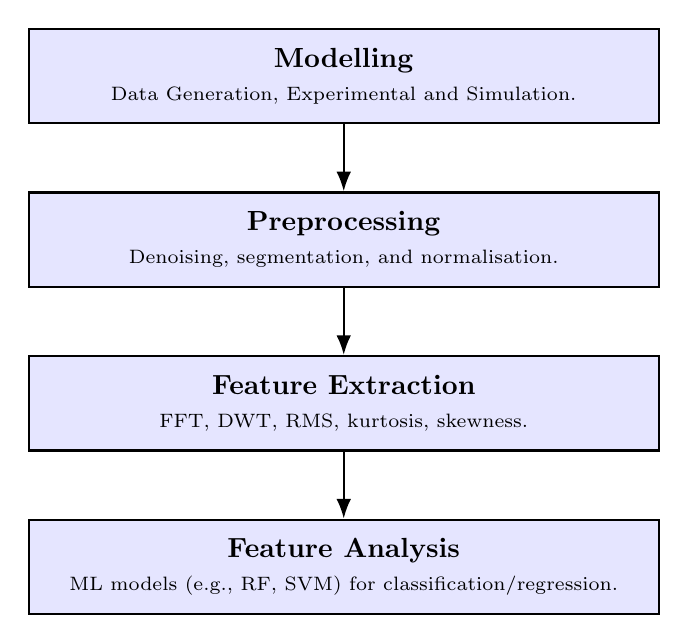
\begin{tikzpicture}[node distance=0.85cm]
        
        % Nodes with reduced height and tighter spacing
        \node[rectangle, draw, thick, minimum width=8cm, minimum height=1.2cm, fill=blue!10, text width=7.7cm, align=center] (model) 
        {\textbf{Modelling} \\ \scriptsize Data Generation, Experimental and Simulation.};
        
        \node[rectangle, draw, thick, below=of model, minimum width=8cm, minimum height=1.2cm, fill=blue!10, text width=7.7cm, align=center] (preprocess) 
        {\textbf{Preprocessing} \\ \scriptsize Denoising, segmentation, and normalisation.};
        
        \node[rectangle, draw, thick, below=of preprocess, minimum width=8cm, minimum height=1.2cm, fill=blue!10, text width=7.7cm, align=center] (extract) 
        {\textbf{Feature Extraction} \\ \scriptsize FFT, DWT, RMS, kurtosis, skewness.};
        
        \node[rectangle, draw, thick, below=of extract, minimum width=8cm, minimum height=1.2cm, fill=blue!10, text width=7.7cm, align=center] (analysis) 
        {\textbf{Feature Analysis} \\ \scriptsize ML models (e.g., RF, SVM) for classification/regression.};
        
        % Arrows
        \draw[-{Latex[length=2.5mm]}, thick] (model) -- (preprocess);
        \draw[-{Latex[length=2.5mm]}, thick] (preprocess) -- (extract);
        \draw[-{Latex[length=2.5mm]}, thick] (extract) -- (analysis);
        
        \end{tikzpicture}
        }
        % \caption*{\scriptsize Sequential stages from simulation to ML-based diagnosis.}
    \end{figure}

\end{frame}

% \begin{frame}{Trade-offs in ML-Based FDD Framework}

%     \begin{figure}[h!]
%         \centering
%         \scalebox{0.75}{ % Adjusted to better fit slide vertically
%         \begin{tikzpicture}[
%             node distance=2.1cm and 1.2cm,
%             box/.style={draw, thick, align=center, minimum width=2.7cm, minimum height=0.9cm},
%             trade/.style={draw=none, font=\scriptsize, align=center, text width=4cm},
%             every edge/.style={draw, thick, -{Latex[length=2.5mm]}}
%         ]
        
%         % Main nodes
%         \node[box, fill=orange!30] (sensitivity) {Sensitivity\\\scriptsize (Early Fault Detection)};
%         \node[box, fill=blue!20, below left=of sensitivity] (robustness) {Robustness\\\scriptsize (Noise \& Load Tolerance)};
%         \node[box, fill=green!30, below right=of sensitivity] (simplicity) {Simplicity\\\scriptsize (Low Model Complexity)};
        
%         % Trade-off arrows
%         \draw[->] (sensitivity) -- node[trade, above left, yshift=-1cm] {↑ Noise Sensitivity\\↓ Robustness} (robustness);
%         \draw[->] (sensitivity) -- node[trade, above right, yshift=-1cm] {↑ Feature Complexity\\↓ Simplicity} (simplicity);
%         \draw[->] (robustness) -- node[trade, below right] {↑ Generalisation\\↓ Fault Resolution} (simplicity);
%         \draw[->] (simplicity) -- node[trade, below left] {↓ Redundancy Handling\\↓ Noise Filtering} (robustness);
%         \draw[->] (simplicity) -- node[trade, above left, yshift=0.7cm, xshift=2.2cm] {↓ Feature Depth\\↓ Weak Fault Detection} (sensitivity);
%         \draw[->] (robustness) -- node[trade, above right, yshift=0.7cm, xshift=-2.2cm] {↑ Smoothing\\↓ Incipient Sensitivity} (sensitivity);
        
%         \end{tikzpicture}
%         }
%     \end{figure}
    
% \end{frame}


    \section{Conclusions}

\begin{frame}
  \frametitle{\textcolor{white}{\bf Conclusions}}


  \begin{itemize}
    \item ....
  \end{itemize}

\end{frame}



    
    \ThankYouFrame

\end{document}